\section{Methodology}
\label{sec:methodology}

\subsection{Benchmarks}
The experiments use three benchmarks that stress different parts of reasoning and planning. GSM8K is a grade-school mathematics benchmark with numeric final answers; in this thesis it primarily serves as a reasoning sanity check and as a sensitive test of prompting and answer-format effects. Countdown-cd4 is a constrained arithmetic planning benchmark in which the model must combine four supplied numbers with arithmetic operations to reach a target; it is the central benchmark for studying whether single-sample and many-sample evaluation produce different model rankings. Trip Planning is a structured natural-language planning benchmark in which the model must produce an itinerary with ordered city visits and exact stay durations; it tests whether the Countdown pattern generalizes from symbolic arithmetic plans to longer text plans that must satisfy a stricter output schema.

\subsection{Models and Prompt Modes}
The comparison uses two masked diffusion language-model families, LLaDA and Dream, and two autoregressive families, Qwen2.5 and Llama~3.1. Each family is evaluated at roughly comparable 7B--8B scale, with base and instruction-tuned variants wherever available. The goal is not to rank isolated checkpoints in the abstract, but to compare how diffusion-style denoising and autoregressive left-to-right sampling behave under the same benchmark, parser, and sample-budget assumptions.

Prompt format is treated as an experimental variable because instruction-tuned checkpoints are typically trained with chat-role templates, while many reasoning benchmarks are written as flat completion prompts. The \texttt{base\_native} mode is used for base checkpoints and leaves the benchmark in its native completion format. The \texttt{instruct\_templated} mode wraps the task in the model's chat template and is the canonical setting for instruction-tuned checkpoints, because it matches their training-time interface. The \texttt{instruct\_flat} mode feeds the same flat benchmark text to an instruction-tuned model without the chat wrapper. It is included as a diagnostic: if a result changes sharply between templated and flat prompting, the measured score reflects prompt-interface sensitivity as well as reasoning ability. This distinction is important for the thesis because Llama-Instruct on GSM8K changes by more than fifty pass@1 percentage points between the two modes while converging at high pass@k.

\subsection{Generation and pass@k Evaluation}
Diffusion runs use fast-dLLM for the main stochastic experiments, while autoregressive runs use vLLM. Deterministic comparisons use temperature $=0$ and one generated sample per question. Stochastic pass@k comparisons use temperature $=0.7$ and generate $16$, $64$, or $128$ samples per question depending on the benchmark and run. GSM8K and Countdown-cd4 use up to $128$ samples in the main comparisons; Trip Planning uses up to $64$ samples because the generations are longer and the parser is stricter.

For each question, let $n$ be the number of generated samples and $c$ the number of samples scored as correct. The pass@k estimator is
\begin{equation}
    \mathrm{pass@}k = 1 - \frac{\binom{n-c}{k}}{\binom{n}{k}}.
\end{equation}
This metric estimates the probability that at least one of $k$ sampled candidates solves the problem. It is therefore a test-time-search metric, not merely another way to report average accuracy. This distinction is central to the thesis: deterministic accuracy asks whether the first answer is strong, while pass@k asks whether a model can explore a set of candidates that contains a correct answer.

\subsection{Parser-Controlled Scoring}
\label{sec:parser-details}
\label{sec:methodology-parsers}
Figure~\ref{fig:parser-pipeline} shows the scoring pipeline. Raw completions are not compared to gold answers directly. They first pass through task-specific extraction and validation rules that convert free-form text into sample-level correctness labels. This parser layer is part of the measurement system: a completion can fail because the reasoning is wrong, because the final answer is in the wrong format, or because the output cannot be parsed into the required plan structure.

\begin{figure}[!htbp]
\centering
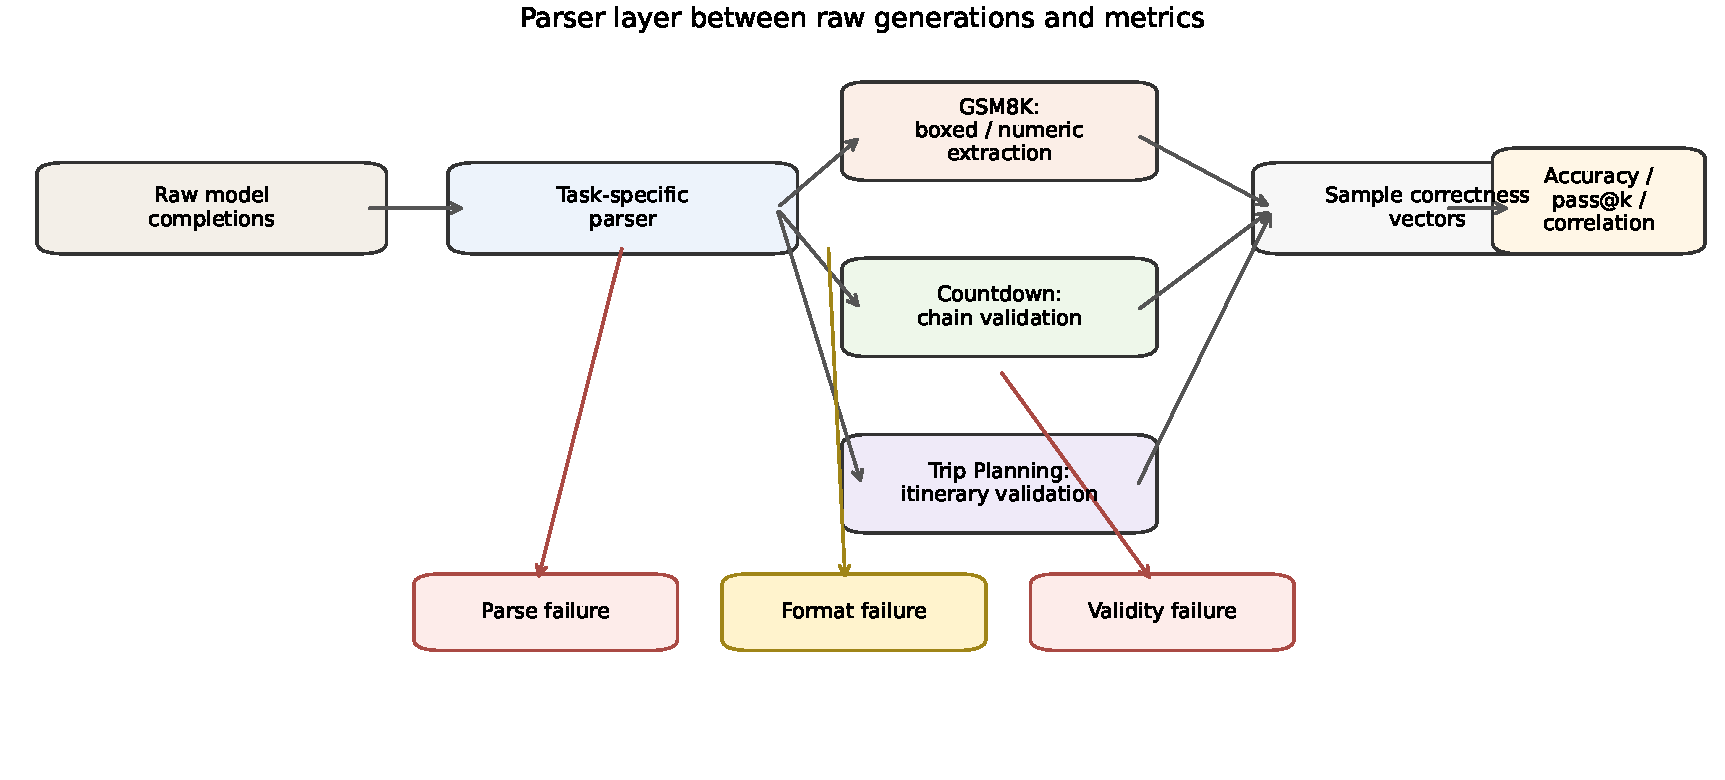
\includegraphics[width=0.98\textwidth]{images/parser_layer_pipeline.pdf}
\caption{Shared evaluation pipeline including the parser layer as an explicit measurement stage. Raw completions are routed through task-specific extractors and validators before sample-level correctness vectors, accuracy, pass@k, and correlation metrics are computed. Parse failure, format failure, and validity failure are analytically distinct outcomes.}
\label{fig:parser-pipeline}
\end{figure}

\textbf{GSM8K.} Gold answers are extracted from the official final-answer marker. Model answers are scored through a boxed-answer extractor, so the canonical evaluation expects the final numeric answer to appear in \texttt{\detokenize{\boxed{...}}} or \texttt{\detokenize{\fbox{...}}}. Commas and numeric formatting are normalized when possible, and numeric predictions are compared against the gold value with a small tolerance. A more permissive final-number fallback is evaluated only as a parser-sensitivity analysis; it is not used to overwrite the canonical scores.

\textbf{Countdown-cd4.} The canonical scorer expects a leading chain of comma-separated binary equations such as \texttt{a+b=c,c-d=e}. The expression chain must evaluate to the target, use only the supplied numbers, use each supplied number at most as often as allowed, and introduce intermediate results only through earlier equations. The allowed operations are addition, subtraction, multiplication, and division after normalizing common operator variants. Invalid syntax, unsafe or unsupported expressions, wrong target values, and wrong number use are scored as failures.

\textbf{Trip Planning.} The Trip Planning scorer parses the generated itinerary for a total-day statement, visit day ranges, and flight lines. From these it reconstructs the ordered city sequence and stay duration for each city, then compares that parsed plan with the required ordered cities and durations. Malformed plans, missing day ranges, missing flight lines, wrong city order, and duration mismatches fail the exact-match validity check.

\subsection{Per-Question Accuracy Analysis}
Average pass@k curves say which model is stronger overall, but they do not reveal whether two models solve the same questions. The per-question analysis therefore computes, for each model and each question, the fraction of generated samples that are correct. Pearson correlations between these vectors quantify failure-mode alignment: high correlation means two models tend to solve and fail on the same questions, while low correlation suggests complementarity.

The same per-question correctness data also supports an oracle-union analysis. This analysis asks how many questions would be solved if an ideal selector could choose from a pair of model families or from all available models. It is not a deployable ensemble, but it gives an upper bound on the value of combining diffusion and autoregressive samples. The generated HTML comparison views are used for qualitative inspection of examples behind these vectors; the thesis reports the numerical correlation and oracle-union results rather than the implementation details of those views.

\subsection{Evaluation Conditions}
The main stochastic comparisons use the same benchmark split, prompt mode, parser, temperature, and sample budget within each condition. GSM8K base and instruct comparisons use $128$ questions and $128$ samples per question; the few-shot ablations use $256$ questions and $16$ samples per question. Countdown-cd4 uses $992$ questions, eight few-shot examples, and $128$ samples per question. Trip Planning uses $200$ questions, two few-shot examples, and $64$ samples per question. Generation length is set to match the task: shorter for Countdown expressions and longer for GSM8K reasoning traces and Trip Planning itineraries. Fixed random seeds are used for sampling and dataset subsampling so that model comparisons within a condition are aligned.
